\documentclass[aspectratio=43]{beamer}
\beamertemplatenavigationsymbolsempty

\mode<presentation>
{
	\usetheme{Singapore}
        \useoutertheme{miniframes}
	%\setbeamercovered{transparent}
	%\setbeamertemplate{footline}[]
        \setbeamertemplate{footline}
                          {
                            \leavevmode%
                            \hbox{%
                              \begin{beamercolorbox}[wd=.333333\paperwidth,ht=2.25ex,dp=1ex,center]{author in head/foot}%
                                \usebeamerfont{author in head/foot}\insertauthor
                              \end{beamercolorbox}%
                              \begin{beamercolorbox}[wd=.333333\paperwidth,ht=2.25ex,dp=1ex,center]{title in head/foot}%
                                \usebeamerfont{title in head/foot}\insertshorttitle
                              \end{beamercolorbox}%
                              \begin{beamercolorbox}[wd=.333333\paperwidth,ht=2.25ex,dp=1ex,right]{date in head/foot}%
                                \usebeamerfont{date in head/foot}\insertshortdate{}\hspace*{2em}
                                \insertframenumber{} / \inserttotalframenumber\hspace*{2ex}
                            \end{beamercolorbox}}%
                            \vskip0pt%
                          }
}

% \usepackage{flashmovie}
\usepackage[utf8]{inputenc}
\usepackage[T1]{fontenc}
%\usepackage[ngerman]{babel}
\usepackage[english]{babel}
\usepackage{amsmath}
\usepackage[absolute,overlay]{textpos}
\usepackage{svg}
\usepackage{xcolor}

\usebackgroundtemplate{%
\begin{tikzpicture}[remember picture,overlay]
\node[anchor=south west] at (current page.south west) {\includegraphics[height=0.4cm]{by.eps}};
\end{tikzpicture}}

\author[]{Anton Kuzmin}
\institute[]{}
\date[FOSDEM 2024]{FOSDEM'24, 3 \& 4 February 2024, Brussels}

\usepackage{tikz}

\title[Filling a Gap]{Filling a Gap Between Hardware and Software\\Cologne Chip GateMate FPGA}

\setbeamerfont{table font}{size=\tiny}

\begin{document}

\begin{frame}
  \titlepage
\end{frame}

\section{Intro}

\begin{frame}
  \frametitle{Who am I\dots}
  \begin{itemize}
  \item not really a software developer\\
    \dots but write code sometimes
  \item developing embedded systems for 25 years
  \item VME, CompactPCI, AdvancedTCA, SoM
  \item FPGA and SoC-FPGA (Altera/Intel, Microsemi/Microchip, Cologne Chip)
  \item VHDL (RTL-code, no, it is not a software)
  \end{itemize}
  \vskip.5cm

%  My usual problem with the software is how to make it run on a
%  hardware which is known not to be working yet and how to bring-up
%  and test this hardware. With a soft-core CPU it is getting even
%  worse.

\end{frame}


\frame{\tableofcontents[subsectionstyle=hide]}

\section{FPGA and software development}

\begin{frame}
\frametitle{Why software develpers should care about FPGA}
\begin{itemize}
  \item conventional hardware architectures are stuck
  \item the only two mainstream HDLs represent software technology
  level of a stone age (well, last century)
\end{itemize}
\vskip.5cm
There should be a way\dots
\vskip.5cm
\begin{itemize}
  \item for reconfigurable hardware to catch up with the progress made
  in the software development world for the last four decades
  \item bring fun and younger generation to FPGA development
\end{itemize}
\end{frame}

\begin{frame}
\frametitle{Current state of FPGA development (for the last 40 years)}
\begin{itemize}
\item RTL and a rise of Verilog and VHDL were a revolition
\item \dots and nothing can compare to it for 40 years
\item may be it is still fine for ASIC
\item \dots but FPGAs are different
\end{itemize}
\end{frame}

\begin{frame}
\frametitle{Two reasons for disappointment (1/2)}
Benefits of reconfigurability at run-time are under-explored and
virtually unexploited
\begin{center}
  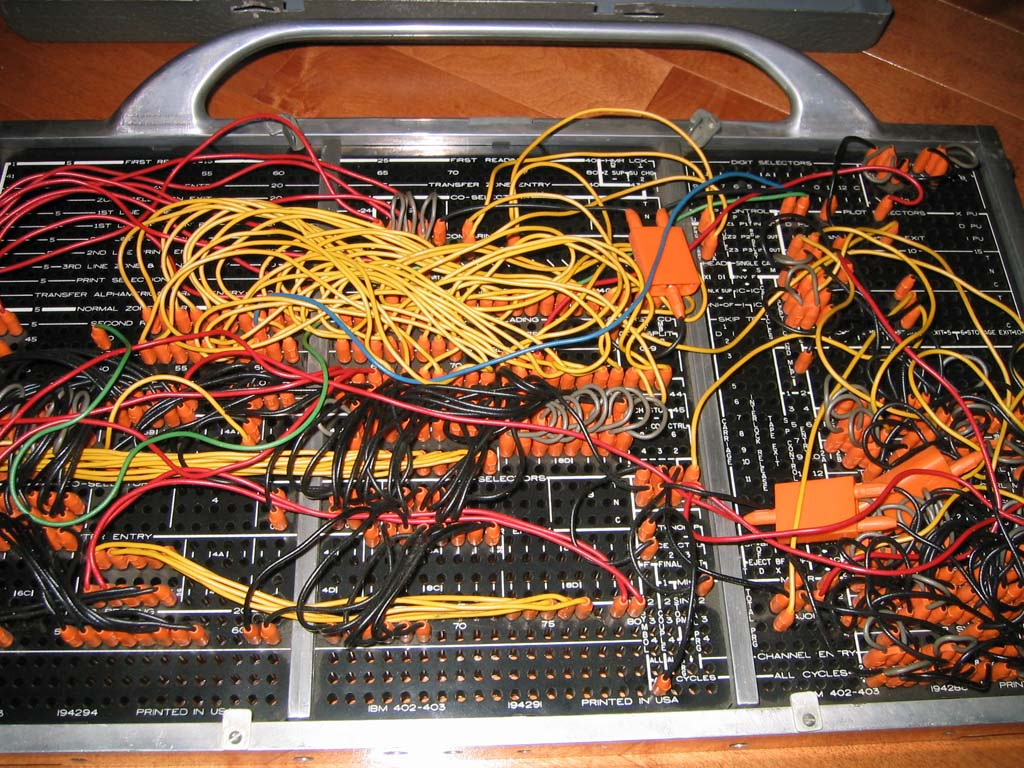
\includegraphics[height=5cm]{IBM402plugboard.Shrigley.wireside.jpg}

  \textcolor{gray}{\tiny{IBM 402 plug-board. Chris Shrigley, 2003, CC-BY}}
\end{center}
\end{frame}

\begin{frame}[t]
\frametitle{Two reasons for disappointment (2/2)}
The only available way is a cross-development
\begin{center}
  \begin{flushleft}
  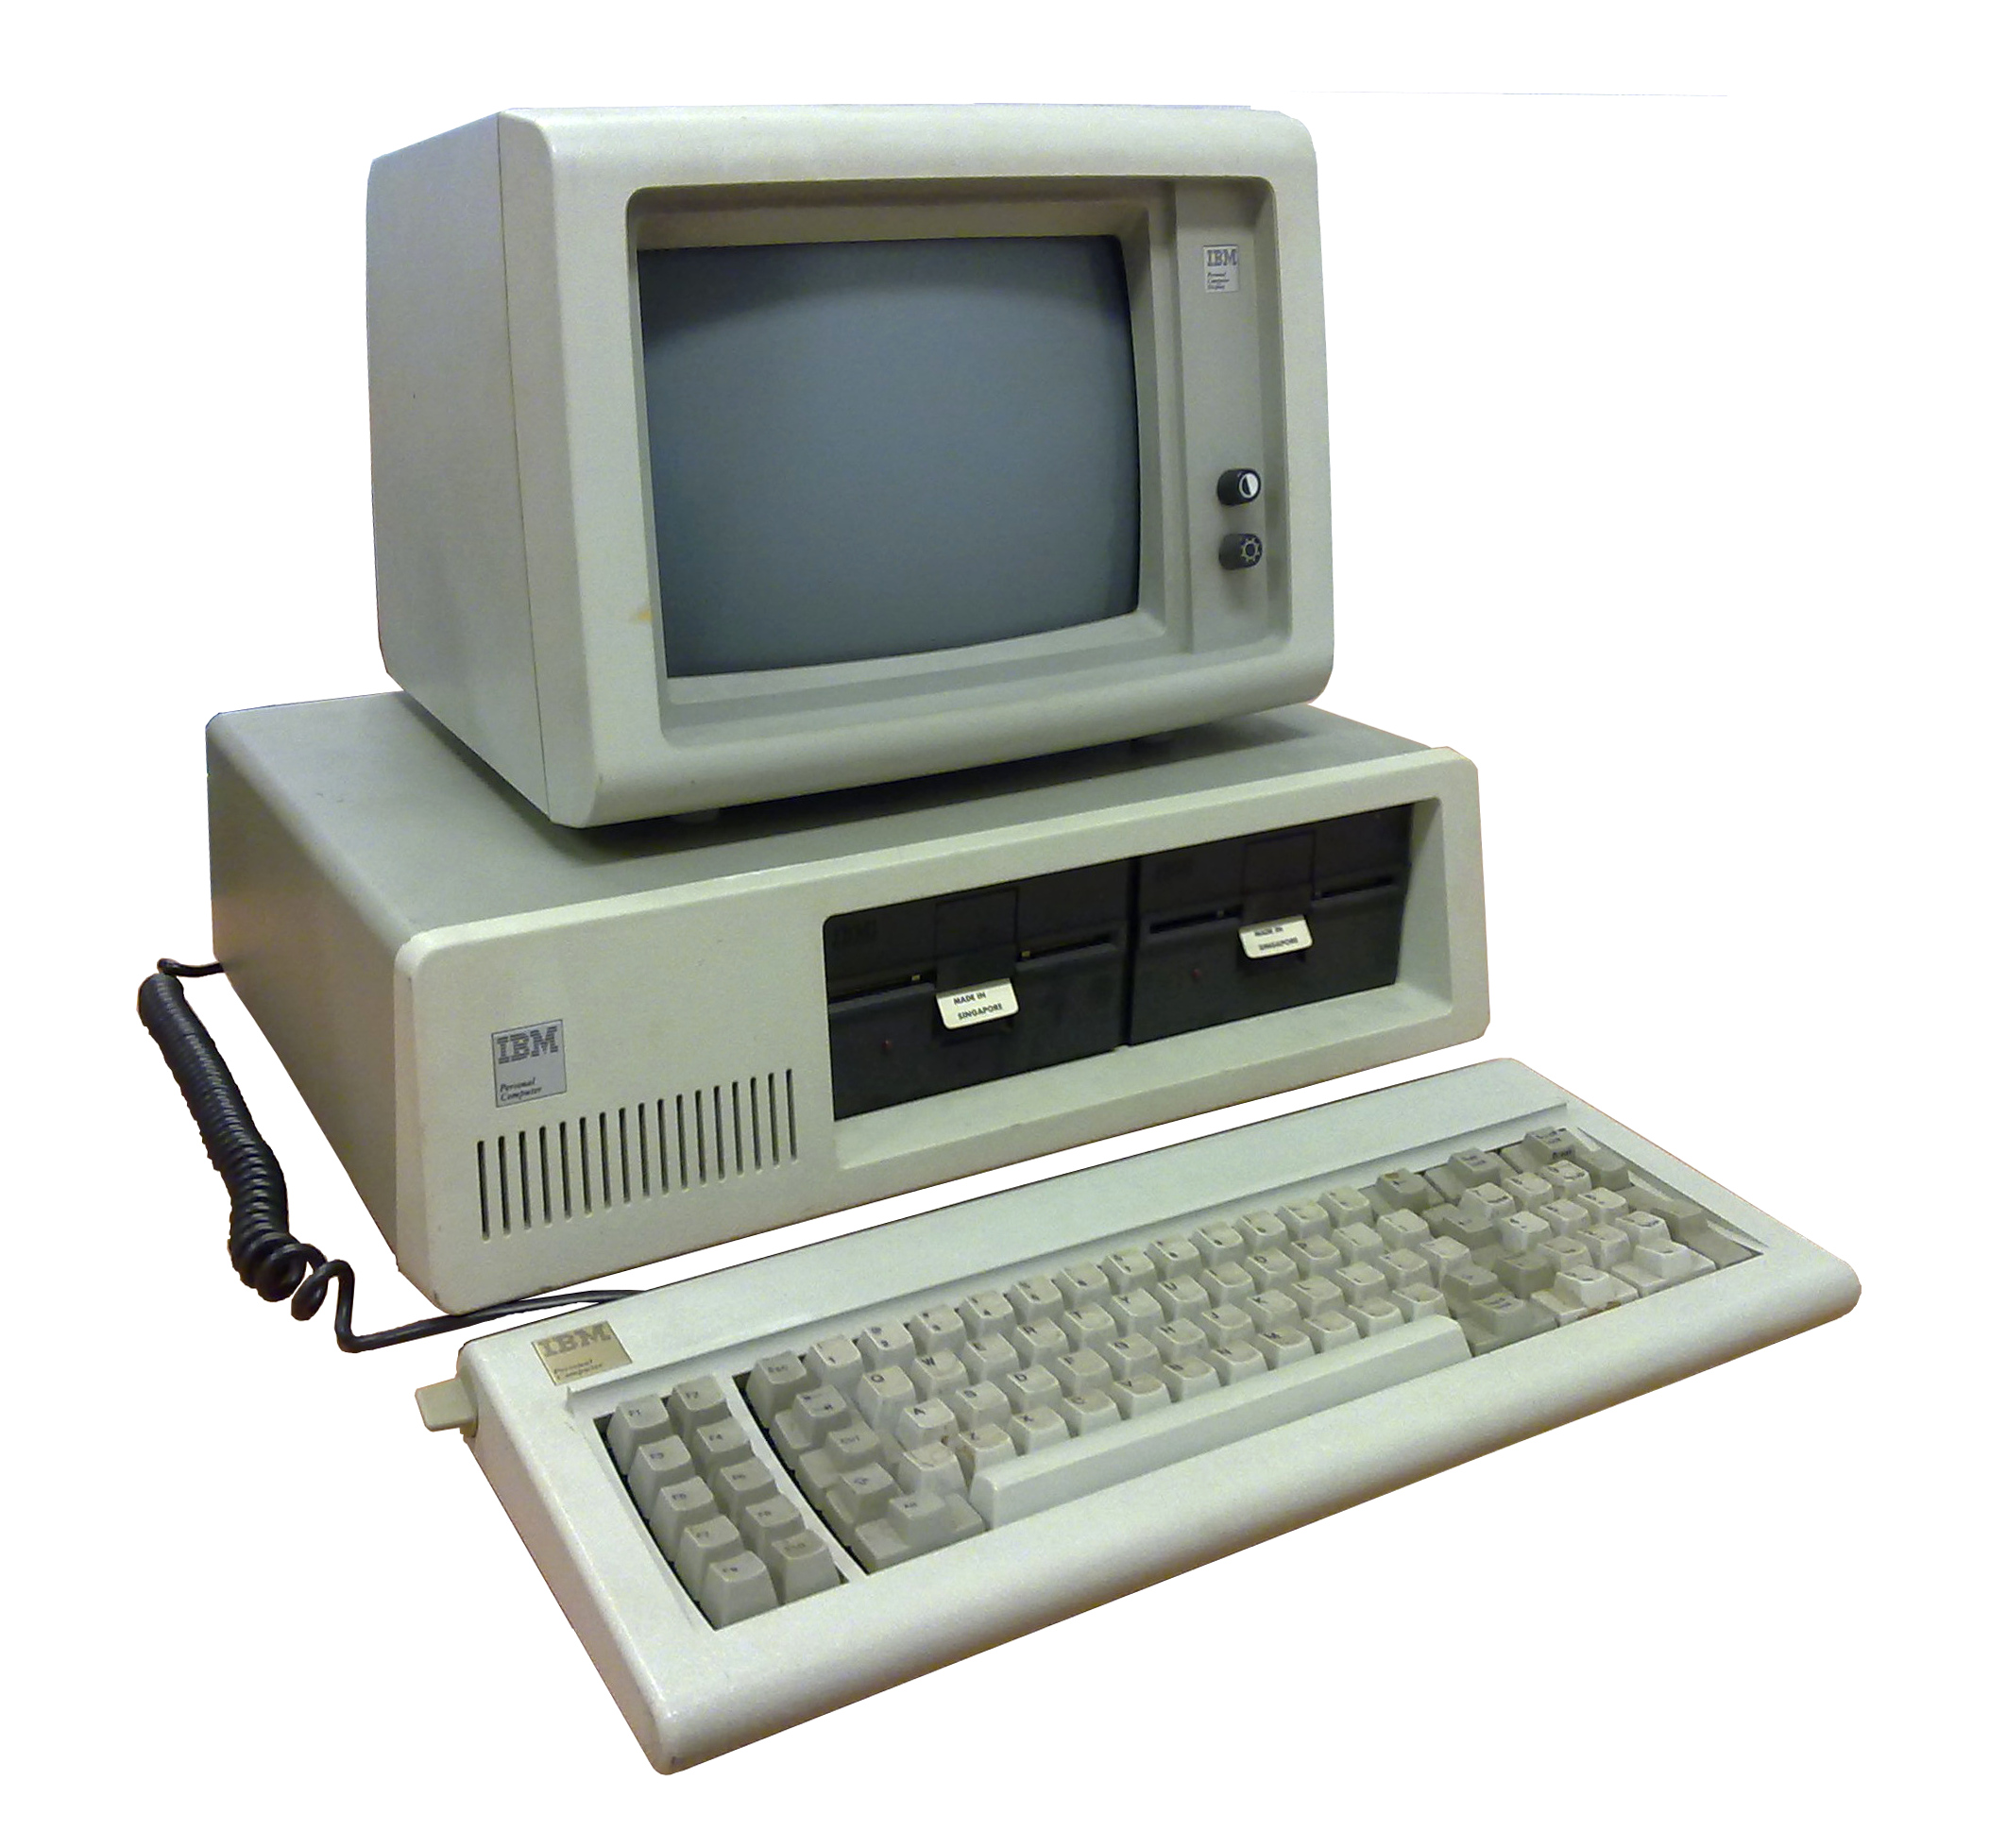
\includegraphics[height=5cm]{Ibm_pc_5150.jpg}

  \textcolor{gray}{\tiny{IBM PC 5150, Ruben de Rijcke, 2010, CC-BY-SA}}
  \end{flushleft}

  \vspace{-4cm}
  \hspace*{4cm}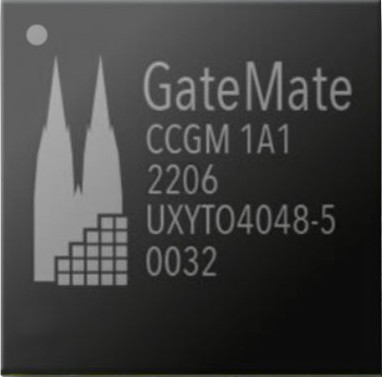
\includegraphics[height=1cm]{CCGM1A1_front.jpg}
\end{center}
\end{frame}

%% ... let's not discuss reasons and complain about it, but see what
%% can be done and why the time is now

%% free tools Yosys and next-pnr
%% open/documented FPGA architecture and bitstream format
%% XC6200, jbit, etc.

\subsection{A Dream of self-hosted FPGA development}

\begin{frame}[t]
\frametitle{Demo\dots}
\vspace{-1cm}
\begin{center}
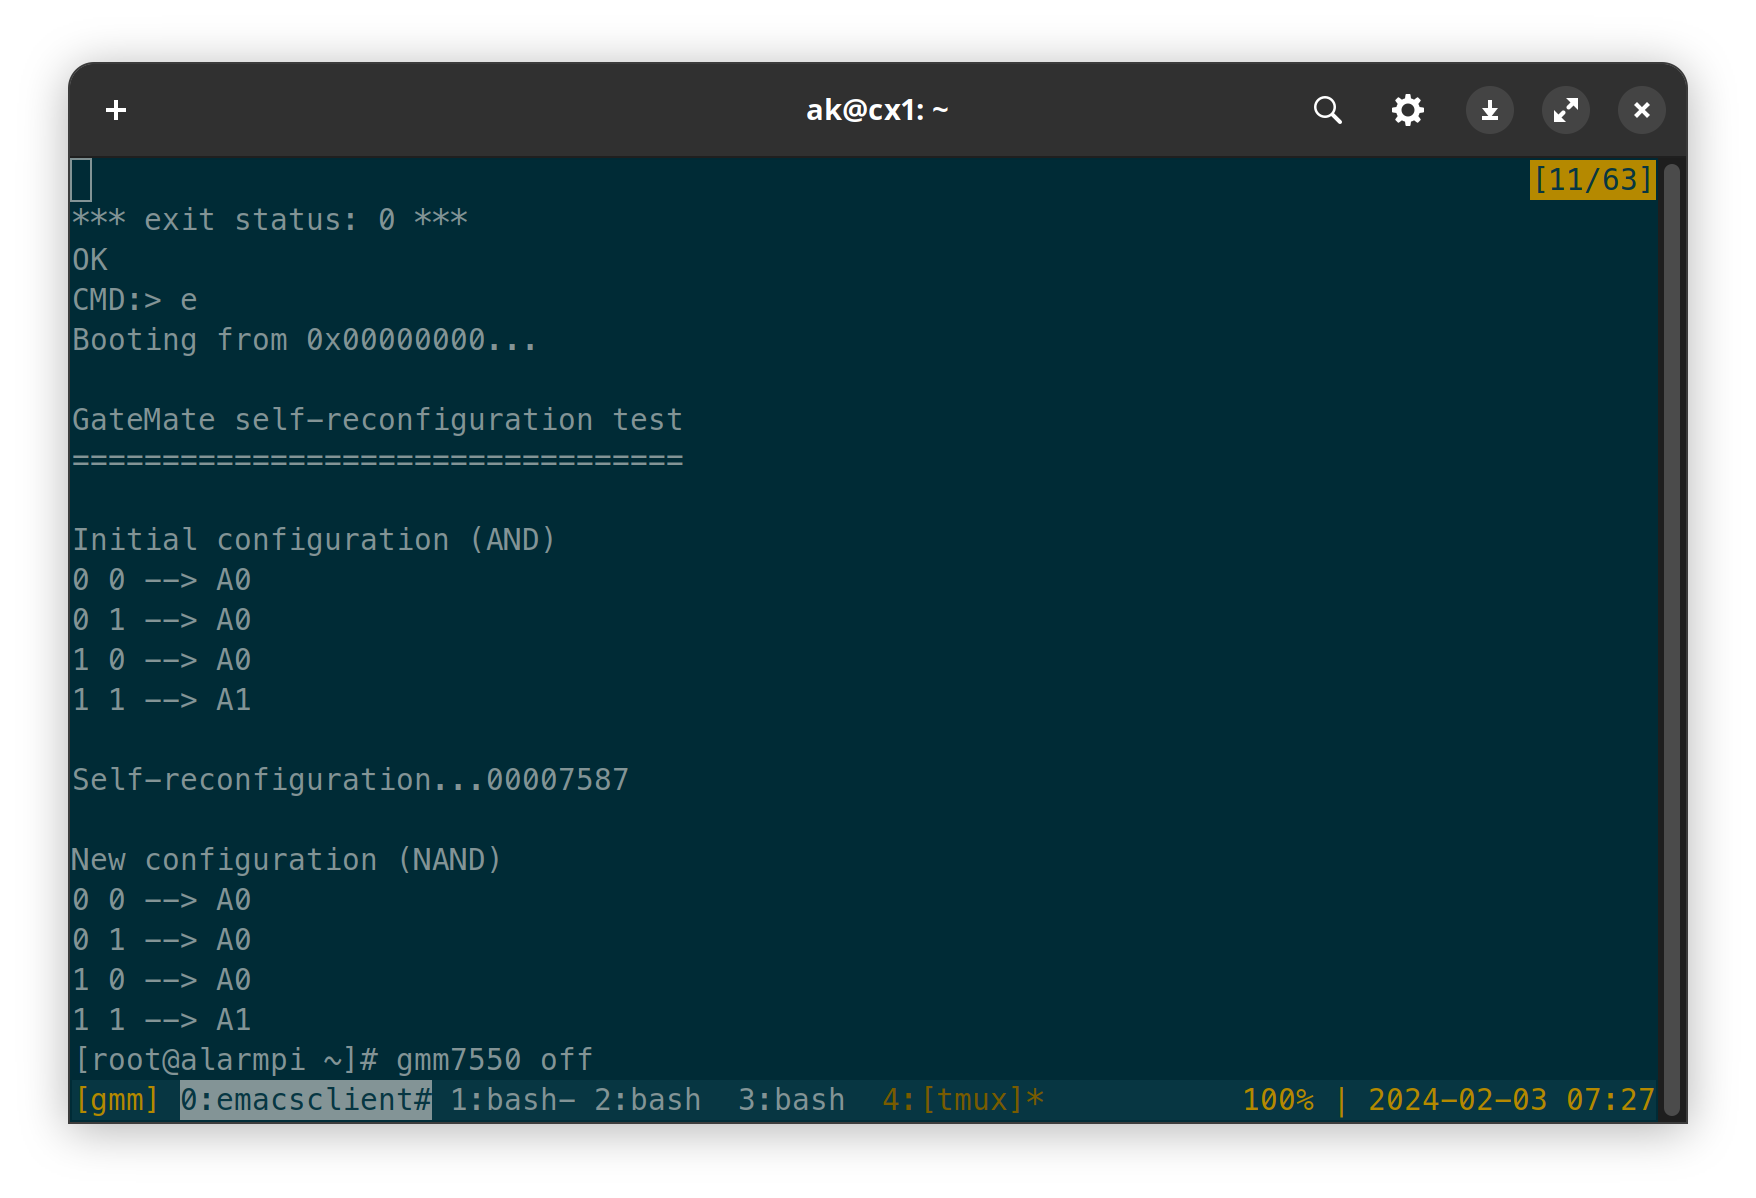
\includegraphics[width=11cm]{screenshot.png}
\end{center}
\end{frame}

\begin{frame}
\frametitle{Perspective}
One small LUT run-time modification to demonstrate, but a huge leap
towards a self-hosted FPGA development.
\begin{itemize}
\item run-time ISA extensions
\item JIT to hardware
\item iterative, interactive, and incremental development
\item encourage exploration and experiments (education)
\item native FPGA development (native is not na\"ive)
\end{itemize}
\end{frame}

\section{Hardware that made it possible}

\subsection{Cologne Chip GateMate FPGA}

\begin{frame}
  \frametitle{GateMate FPGA Architecture (1/3)}
  \begin{itemize}
  \item novel CPE architecture (8-input LUT tree, two flip-flops or latches)
  \item low power consumption (GlobalFoundries 28~nm SLP (Super Low
  Power) process)
  \item 4 programmable PLL
  \item dual-ported block RAM
  \item 5 Gbps SerDes
  \item configuration via QSPI up to 100 MHz
  \item all pins configurable as single-ended (1.2 .. 2.5V) or LVDS
  \item all GPIO blocks support DDR
  \item 324-ball BGA, 15x15mm
  \end{itemize}
\end{frame}

\begin{frame}
  \frametitle{GateMate FPGA Architecture (2/3)}

  \begin{center}
    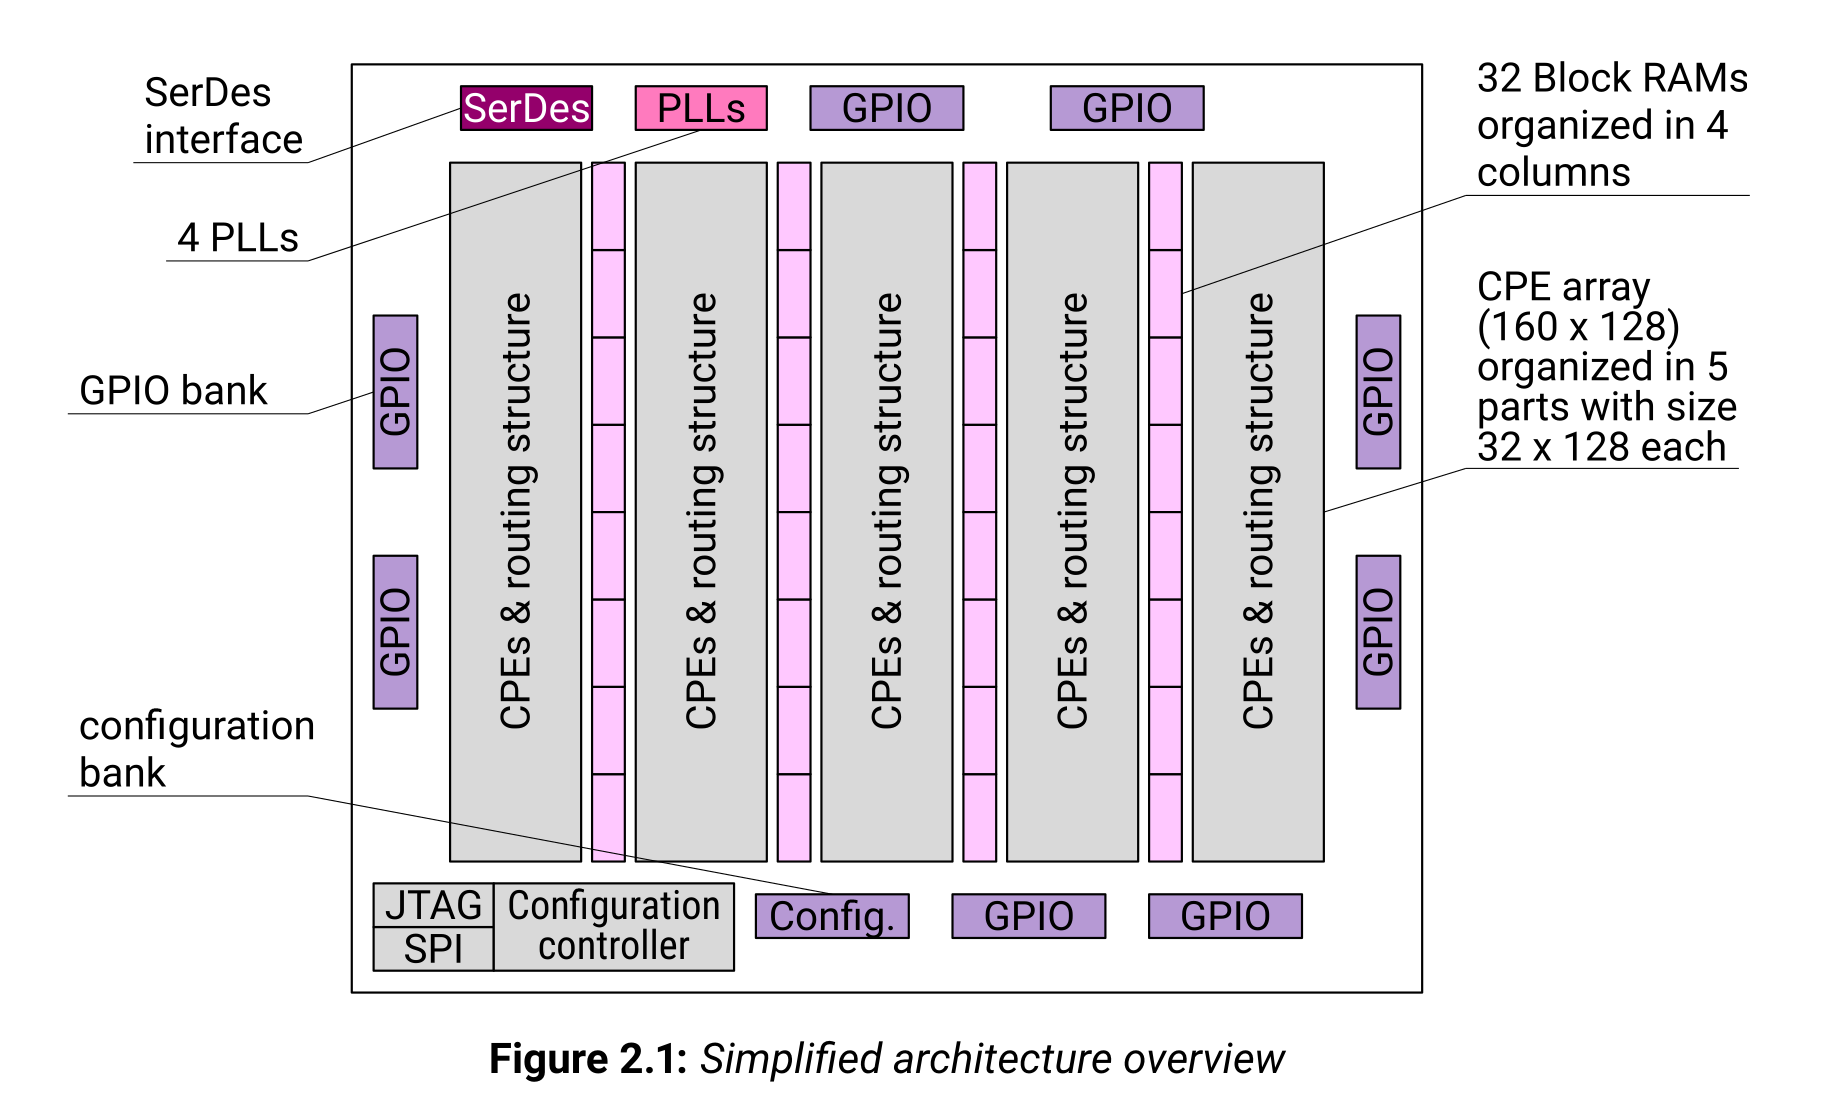
\includegraphics[height=6.5cm]{Figure_2.1.png}

    \footnotesize{{CologneChip~GateMate} FPGA Datasheet, DS1001, January 2023, page 21}
\end{center}
\end{frame}

\begin{frame}
  \frametitle{GateMate FPGA Architecture (3/3)}
  \vspace{-.5cm}
  \begin{center}
    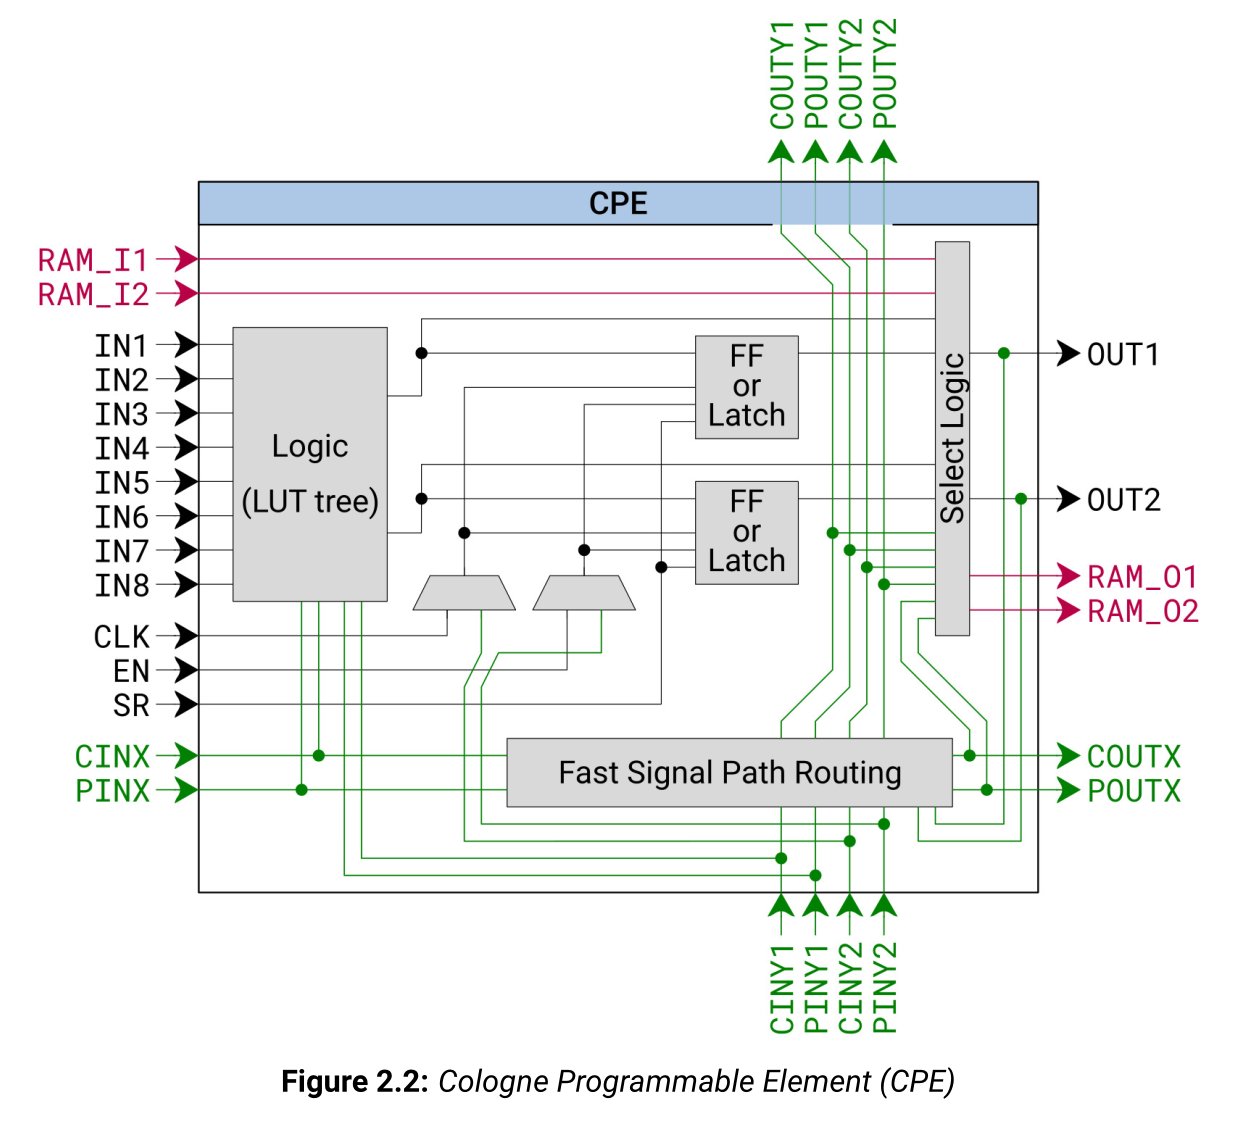
\includegraphics[height=6.5cm]{Figure_2.2.png}

    \footnotesize{{CologneChip~GateMate} FPGA Datasheet, DS1001, January 2023, page 22}
  \end{center}
\end{frame}

\subsection{GMM-7550 Module}

\begin{frame}
  \frametitle{Why to design a module}

  \begin{flushright}
    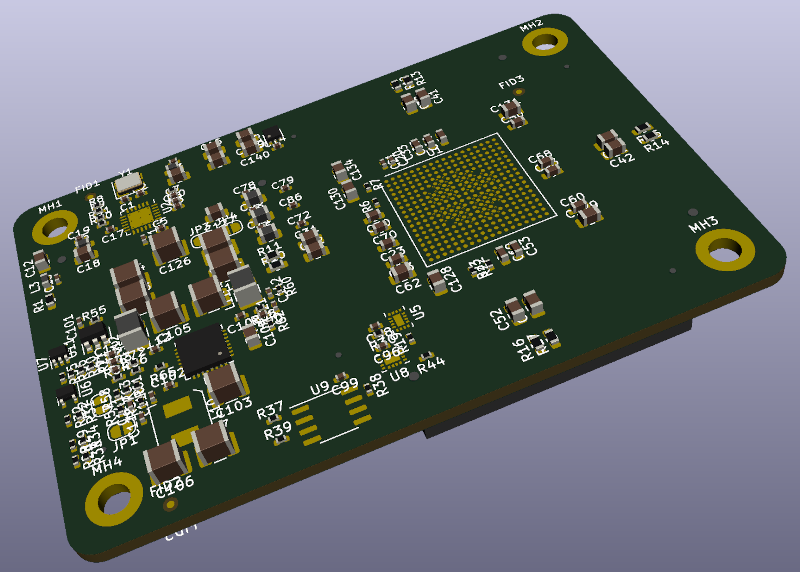
\includegraphics[height=3cm]{GMM-7550_preview_2020-10-01.png}
  \end{flushright}
  \vspace{-4cm}

  \begin{minipage}{6.5cm}
  \begin{itemize}
    \item CCGM1A1 is the best thing since XC6200
    \item an Evaluation Kit was not available back in mid-2020
    \item a module is smaller and reusable
    \item freedom for experiments\\(e.g. to interconnect several FPGAs)
    \item best way to get to know a new chip
  \end{itemize}
  \end{minipage}
  \begin{itemize}
    \item fun and easy exercise with KiCAD\\(at least it seemed so at
  the beginning)
  \end{itemize}
\end{frame}

\begin{frame}
  \frametitle{Current Status}
  \begin{itemize}
    \item three boards designed and manufactured
    \item the boards are functional (from the very first versions and
    with just a few minor problems)
    \item schematic symbol and PCB footprint for GateMate FPGA are accepted
    into KiCAD v7 libraries
    \item control application is functional enought to debug, test,
    and configure the module
    \item several VHDL examples are running
    \item support for the module is (to be) added to the FuseSoC and LiteX
    (work in progress, nothing is upstreamed yet)
    \item \dots it took roughly 5 times longer than initially estimated
  \end{itemize}
\end{frame}

\begin{frame}
  \frametitle{GMM-7550 Module}

  \begin{flushright}
    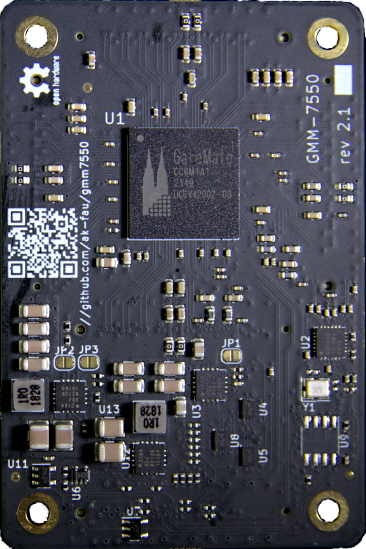
\includegraphics[height=5cm]{gmm7550.jpg}
  \end{flushright}
  \vspace{-5.5cm}

  \begin{minipage}{7.5cm}
  \begin{itemize}
  \item Cologne Chip GateMate FPGA CCGM1A1
  \item wide-range input power
  \item module control: discrete signals and I$^2$C
  \item 8 I/O banks available on 4 connectors\\with identical pinout
  \item 5 Gbps SerDes
  \item programmable clock
  \item all configuration modes are supported\\(Active and Passive SPI,
  and JTAG)
  \end{itemize}
  \end{minipage}
\end{frame}

\subsection{Accessories}

\begin{frame}
  \frametitle{Raspberry-Pi 40-pin GPIO HAT Adapter}
  \vspace{1cm}
  \begin{flushright}
    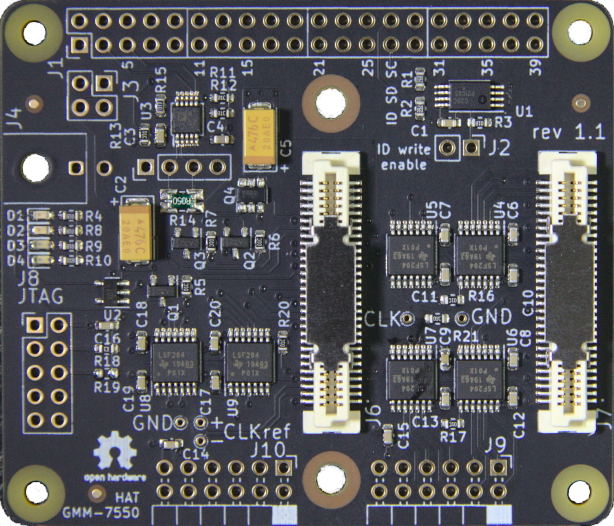
\includegraphics[angle=90, height=3.5cm]{hat-gmm7550.jpg}
  \end{flushright}
  \vspace{-6cm}

  \begin{minipage}{8cm}
  \begin{itemize}
  \item power for the module from R-Pi 5V or a separate power connector
  \item current and voltage monitoring (ADM1177)
  \item module control signals, I$^2$C, SPI, and UART
  \item 2x5 .1'' JTAG connector
  \item 2.5V/3.3V I/O level converters
  \item two 12-pin P-mod connectors for extension modules
  \item access to 3 I/O connectors
  \item 4x LEDs
  \item R-Pi HAT ID EEPROM
  \end{itemize}
  \end{minipage}
\end{frame}

\begin{frame}
  \frametitle{Memory Extension Module}

  \begin{minipage}{9cm}
  \begin{itemize}
  \item SRAM 512K x8 (CY7C1049GN30-10ZSXI)
  \item QSPI-NOR 128Mb (16MiB, IS25LP128-JBLE)
  \vspace{.5cm}
  \item mechanical design validation
  \end{itemize}
  \end{minipage}

  \vspace{-1cm}
  \begin{flushright}
    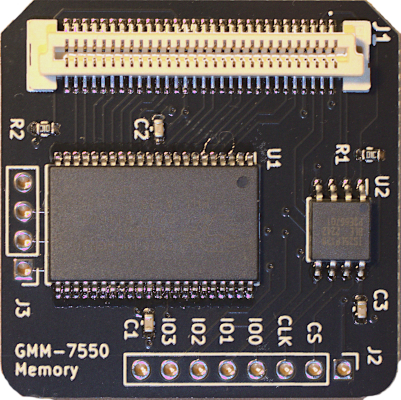
\includegraphics[height=3cm]{mem-module.jpg}
  \end{flushright}

\end{frame}

\section{Road ahead}

\begin{frame}
\frametitle{It doesn't have to be\dots}
It \textbf{has} to be Cologne Chip GateMate (at least for now),\\
but it does not have to be\dots
\begin{itemize}
\item RISC-V (it is still a good choice)
\item C (anything else would be better)\\Forth, Lua, microPython,
Scheme, Scala, Rust, \dots
\item GMM-7550 module\\CologneChip Evaluation board, Trenz, Olimex
\end{itemize}
\end{frame}

\begin{frame}
  \frametitle{You are invited to innovate\dots}

  The greatest engineering reward and pleasure is to see the results
  used, so, please:

  \vspace{.5cm}

  \begin{itemize}
  \item create software for FPGAs and with FPGAs
  \item build modules, design baseboards and extension modules
  \item report problems
  \item create custom designs
  \item experiment
  \item share
  \end{itemize}

  \vspace{-2cm}
  \begin{flushright}
    \includesvg[height=3cm]{oshw-logo.svg}
  \end{flushright}

\end{frame}

\section{Contact info}
\begin{frame}

  \begin{minipage}{7cm}
    \vskip.5cm
    \huge{Thank you!}
    \vskip1cm
    \small{Anton Kuzmin}\\
    \small{\texttt{ak@gmm7550.dev}}\\
    \small{\texttt{https://github.com/gmm-7550/}}
    \vskip.5cm
    \Huge{Questions?..}
  \end{minipage}

  \vspace{-5cm}
  \begin{flushright}
    \includegraphics[height=5cm]{gmm7550-vcard.png}\\
  \end{flushright}

\end{frame}


\section{Backup slides}

\begin{frame}
  \frametitle{GMM-7550 Module -- Power}
  \begin{itemize}
  \item wide input range (2.9 .. 6.5V), may be powered directly from a
  3.3V baseboard, 5V USB, or single cell Li-Pol
  \item DC-DC are synchronized to the base clock and run in
  counter-phase\\(default 1.25~MHz, PLL programming option)
  \item 0.9/1.0/1.1V V$_{\text{core}}$ (build-time option)
  \item V$_{\text{io}}$ may be supplied directly on the module (2.5V, build-time
  option) or from\\a baseboard (individually for each I/O bank)
  \item ADP2164 step-down DC-DC, V$_{\text{io}}$ (2.5V) and V$_{\text{core}}$ are rated up to 4A
  \item separate LDO (ADP1753) for SerDes and SerDes PLL, 1.0/1.1V, 800mA
  \item input voltage monitor/reset generator on the module, an
  external reset input, and I$^2$C controllable reset
  \end{itemize}
\end{frame}

\begin{frame}
  \frametitle{GMM-7550 Module -- Clock}
  \begin{itemize}
  \item Texas Instruments CDCE6214 PLL with internal EEPROM
  \item 25~MHz crystal on the module
  \item LVDS reference clock input
  \item single-ended (LVCMOS 2.5V) and two differential output clocks
  \item default 100~MHz differential clock to the FPGA \texttt{SER\_CLK} input
  \item dedicated output for DC-DC synchronization
  \end{itemize}
\end{frame}

\begin{frame}
  \frametitle{GMM-7550 Module -- FPGA Configuration}
  \begin{itemize}
  \item JTAG (2.5V) available on the module connector
  \item Active Serial mode from SPI-NOR on the module or on a
  baseboard
  \item Passive Serial mode from a baseboard
  \item configuration mode and SPI connection configurable via I$^2$C
  \item SPI-NOR on the module is accessible from a baseboard
  \item \textbf{default mode:} Active Serial from SPI-NOR on the module
  \end{itemize}
\end{frame}

\end{document}
